% Document class and parameters %
\documentclass[10pt,a4paper]{article}
% Document packages %
\usepackage{graphicx}
\usepackage{biblatex}
\usepackage{parskip}
\usepackage{listings}
\usepackage{caption}
\usepackage{subcaption}
\usepackage{amsmath}
\usepackage[most]{tcolorbox}


\graphicspath{{./Images/}}
\setlength{\parskip}{1em}

% Document Body %
\begin{document}
\begin{titlepage}
	\centering
	{\scshape\LARGE Imperial College London \par}
	\vspace{1cm}
	{\scshape\Large Mathematics: Year 2\par}
	\vspace{1.5cm}
	{\huge\bfseries Joint Distributed Random Variables \par}
	\vspace{2cm}
	{\Large\ Xin Wang }
	\vfill
	{\large \today\par}
\end{titlepage}

\begin{abstract}
	In Statistics, the two most important but difficult to understand concepts are Law of Large
	Numbers (LLN) and Central Limit Theorem (CLT). These form the basis of the popular hypothesis
	testing framework. In the practical world, its impossible to analyse an entire population.
	Hence, mathematicians resort to sampling from the population, perform analysis and draw
	conclusions about the population based on the sample.
	
\end{abstract}

\tableofcontents
\pagebreak

%%%%%%%%%%%%%%%%%%%%%%%%%%%%%%%%%%%%%%%%%%%%%%%%%%%%%%%%%%%%%%%%%%%%%%%%%%%%%%%%%%%%%%%%%%%%%%%%%%%%%%%%%%
% Sections Body %
\section{Introduction}

It is understood intuitively that the average of many measurements of the same unknown quantity
tends to  give a better estimate than a single measurement. This is because the random error of
each measurement cancels out in the average.  In thi section, this intuition is precisely
defined in two ways: the law of large numbers (LoLN) and the central limit theorem (CLT).

The random variables $X_i$ evaluated are \textbf{independent and identically distributed}. This
means that random variables $X_1,X_2,\dots,X_n$  are independent and have the \textbf{same underlying
distribution}. 

The random variables that are independent and identically distributed satisfies the following properties:
\begin{enumerate}
	\item Random variables $X_1,\dots,X_n$ are all independent.
	\item Random variables have the same expectation 
	$$E(X_i) = \mu$$ 
	$\forall i$ where $\mu$ is the mean.
	\item Random variables have the same variance 
	$$\text{Var}(X_i) = \sigma^2$$
	$\forall i$ where $\sigma^2$ is the variance and $\sigma$ is the standard deviation.
\end{enumerate}

As a breif   the law of large numbers and central limit theorem are based on \textbf{the multiple
independent samples from the same distribution}. 

The LoLN shows two conclusions:
\begin{itemize}
	\item The average of many independent samples is (with high probability) close to the mean of the
	underlying distribution.
	\item The density histogram of many independent samples is (with high probability) close to the graph of the density of the underlying distribution.
\end{itemize}

The central limit theorem says that the average of many independent copies of a random
variable is \textbf{approximately a normal random variable}. The CLT goes on to give precise values for the
mean and standard deviation of the normal variable.

It should be noted that mathematics cannot tell us if the experiment is producing data worth
averaging. For example, if the measuring device is defective or poorly calibrated then the average
of many measurements will be wrong even if the experiment is highly accurate. This  is  an  example
of \textbf{systematic error or sampling bias}, as opposed to the random error which can be
controlled by the law of large numbers.

\pagebreak
%%%%%%%%%%%%%%%%%%%%%%%%%%%%%%%%%%%%%%%%%%%%%%%%%%%%%%%%%%%%%%%%%%%%%%%%%%%%%%%%%%%%%%%%%%%%%%%%%%%%%%%%%%
\section{Law of large numbers}

As mentioned previously,$X_i$ are independent and identically-distributed thus $X_i$ all have the
same mean $\mu$ and standard deviation $\sigma$.

Let $\overline{X}_n$ be a random variable and the average of $X_1,\dots,X_n$:
\begin{align*}
	\overline{X}_n = \frac{X_1+X_2+\dots+X_n}{n} = \frac{1}{n}\sum_{i=1}^n X_i
\end{align*}
The law of large numbers and central limit theorem takes $\overline{X}_n$ and shows the value
and distribution of $\overline{X_n}$ respectively.
\begin{itemize}
	\item LoLN: As $n$ grows, the probability that $X_n$ is close to $\mu$ goes to 1.
	\item CLT: As $n$ grows, the distribution of $X_n$ converges to the normal distribution
	$N(\mu,\frac{\sigma^2}{n})$
\end{itemize}

\textbf{Example 1}: Averages of Bernoulli random variables

\textbf{Bernoulli variable}: A random variable that takes value 1 in case of success and 0 in case of failure.

Suppose each $X_i$ is an independent flip of a fair coin
\begin{align*}
	X_i &\sim \text{Bernoulli(0.5)} \\
	\mu &= 0.5
\end{align*}
$\overline{X}_n$ is the proportion of H in $n$ flips, and it is expected that this proportion is
close to $0.5$ for large $n$ since $\mu = 0.5$. However, note that due to the nature of randomness,
this is not guaranteed e.g. it is possible to get 1000 H in 1000 flips, though the probability is
very small. 

A more accurate definition of this intuitive idea is: \textbf{There is with high
probability} the sample average $\overline{X}_n$ is close to the mean 0.5 for large $n$.

\textbf{Proof}: Investigate the probability of th sample average $\overline{X}_n$ being within $0.1$
of the mean $\mu$ $0.5$.
\begin{align*}
	P(|\overline{X}_n - 0.5|<0.1) \; \text{or equivalently} \; P(0.4 \leq \overline{X}_n \leq 0.6)
\end{align*}
The law of large numbers says that this probability goes to 1 as the number of flips $n$ gets large.
This is seen through any program used to calculate the binomial probability distribution $P(0.4 \leq
\overline{X}_n \leq 0.6)$:
\begin{figure} [h!]
	\centering
	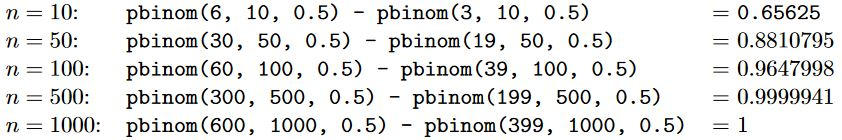
\includegraphics[scale=0.62]{pbino.JPG}
	\caption{R code producing the following values for $P(0.4 \leq\overline{X}_n \leq 0.6)$}
\end{figure}

The law of large numbers still apply with the probability of being within $0.01$ of the mean. It
will take larger values of $n$ to raise the probability to near 1. 
\begin{figure} [h!]
	\centering
	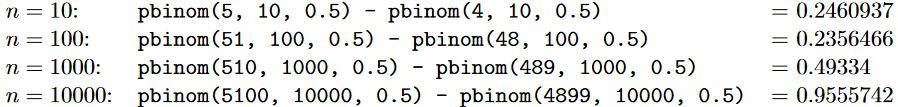
\includegraphics[scale=0.62]{pbino2.JPG}
	\caption{R code producing the following values for $P(0.49 \leq\overline{X}_n \leq 0.51)$}
\end{figure}

This convergence of the probability to 1 is proof of the LoLN. 

%%%%%%%%%%%%%%%%%%%%%%%%%%%%%%%%%%%%%%%%%%%%%%%%%%%%%%%%%%%%%%%%%%%%%%%%%%%%%%%%%%%%%%%%%%%%%%%%%%%%%%%%%%
\subsection{Formal statement of the law of large numbers}

Given that random variables $X_1,X_2,\dots,X_n$ are independent and share identical distribution
with mean $\mu$ and variance $\sigma^2$, for each $n$, let $X_n$ be the average of the first $n$ variables.

\begin{tcolorbox}[breakable,colback=white]
	For any $a >0$
	\begin{align*}
		\lim_{n \rightarrow \infty} P(|\overline{X}_n - \mu|<a) = 1
	\end{align*}
\end{tcolorbox}

The equation precisely defines that as $n$ increases the probability of being within $a$ of the mean
goes to 1 where $a$ is a small tolerance of error from the true mean $\mu$. If the tolerance $a$ is
decreased or the probability $p$ is increased, then $N$ will need to be larger. For example, in the
previous example, if the probability that the proportion of heads $X_n$ is within $a= 0.1$ of
$\mu=0.5$ is to be at least $p= 0.99999$, then $n > N=500$ is large enough.

%%%%%%%%%%%%%%%%%%%%%%%%%%%%%%%%%%%%%%%%%%%%%%%%%%%%%%%%%%%%%%%%%%%%%%%%%%%%%%%%%%%%%%%%%%%%%%%%%%%%%%%%%%
\subsection{Binomial distribution and normal distribution}

Suppose we have n random variables, $X_i$ for $i = 1, 2,\dots, n$, mutually independent and
identical i.e. the same distribution, each having mean $\mu$ and variance $\sigma^2$:
\begin{align*}
	E\left(\sum_{i=1}^n X_i\right) &= \sum_{i=1}^n E(X_i) = n\mu \\
	\text{Var}\left(\sum_{i=1}^n E(X_i)\right) &= \sum_{i=1}^n \text{Var}(X_i) = n\sigma^2
\end{align*}
It can be shown that, as $n \rightarrow \infty$ the distribution of this sum converges to the normal
distribution:
\begin{align*}
	X_1 + X_2 + \dots + X_n \rightarrow N(n\mu, n\sigma^2) 
\end{align*}

\pagebreak
%%%%%%%%%%%%%%%%%%%%%%%%%%%%%%%%%%%%%%%%%%%%%%%%%%%%%%%%%%%%%%%%%%%%%%%%%%%%%%%%%%%%%%%%%%%%%%%%%%%%%%%%%%
\section{Central Limit Theorem}

\begin{tcolorbox}[breakable,colback=white]
\textbf{Central Limit Theorem}: No matter what the shape of the population distribution is, the
sampling distribution of the sample means approaches a normal distribution as the sample size $n$ gets
larger.
\end{tcolorbox}
 
Graphically speaking, the CLT can be illustrated with rolling a fair die. The more times the die is
rolled, the more likely the shape of the distribution of the means tends to look like a normal
distribution graph.

\begin{figure} [h!]
	\centering
	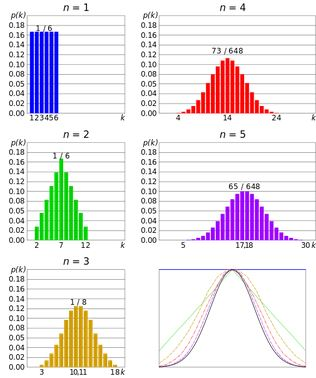
\includegraphics[]{CLT.JPG}
\end{figure}

An essential component of the Central Limit Theorem is that the average $\mu$ of the sample will be
the population mean $\mu$. Similarly, if by finding the average of all of the standard deviations in
the sample, the actual standard deviation $\sigma$ for your population is found.


%%%%%%%%%%%%%%%%%%%%%%%%%%%%%%%%%%%%%%%%%%%%%%%%%%%%%%%%%%%%%%%%%%%%%%%%%%%%%%%%%%%%%%%%%%%%%%%%%%%%%%%%%%
\subsection{Standardisation}

Given a random variable $X$ with mean $\mu$ and standard deviation $\sigma$, standardisation of $X$
is defined as a new random variable: 
\begin{align*}
	Z = \frac{X-\mu}{\sigma}
\end{align*}
Note:
\begin{itemize}
	\item $Z$ has mean of 0 and standard deviation of 1.
	\item  if $X$ has a normal distribution, then the standardization of $X$ results in the standard normal
	distribution $Z$
\end{itemize}  

%%%%%%%%%%%%%%%%%%%%%%%%%%%%%%%%%%%%%%%%%%%%%%%%%%%%%%%%%%%%%%%%%%%%%%%%%%%%%%%%%%%%%%%%%%%%%%%%%%%%%%%%%%
\subsection{Statement of the central limit theorem}

Suppose $X_1,X_2,\dots,X_n$, are independent and share the identical distribution, the random
variables each having mean $\mu$ and standard deviation $\sigma$. 

For each $n$ let $S_n$ denote the sum of $X_1,X_2,\dots,X_n$:
\begin{align*}
	S_n = X_1 + X_2 + \dots + X_n = \sum_{i=1}^n X_i 
\end{align*}
and let $X_n$ denote the average of $X_1,\dots,X_n$:
\begin{align*}
	\overline{X}_n = \frac{X_1 + X_2 + \dots + X_n}{n} = \frac{S_n}{n} 
\end{align*}

The properties of mean and variance for both $S_n$ and $\overline{X}_n$ are defined as:
\begin{figure} [h!]
	\centering
	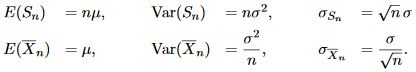
\includegraphics[scale=0.9]{meanandvariance.JPG}
\end{figure}

Notice that the mean and variance for both $S_n$ and $\overline{X}_n$ are multiples of each other
thus both would have the same standardisation:
\begin{align*}
	Z_n = \frac{S_n - n\mu}{\sigma \sqrt{n}} = \frac{\overline{X}_n - \mu}{\frac{\sigma}{\sqrt{n}}}
\end{align*}

This leads to the Central Limit Theorem:
\begin{equation*}
	\overline{X}_n \approx N(\mu, \frac{\sigma^2}{n}) \qquad S_n \approx N(n\mu,n\sigma^2) \qquad Z_n \approx N(0,1)
\end{equation*}
These three equations show:
\begin{itemize}
	\item $\overline{X}_n$ is approximately a normal distribution with the same mean as $X$	but a smaller variance.
	\item $S_n$ is approximately normal.
	\item Standardized $\overline{X}_n$ and $S_n$ are approximately standard normal.
\end{itemize}

The central limit theorem is used to approximate a sum or average of i.i.d random variables by a
normal random variable. This is extremely useful because it is usually easy to do computations with
the normal distribution.

%%%%%%%%%%%%%%%%%%%%%%%%%%%%%%%%%%%%%%%%%%%%%%%%%%%%%%%%%%%%%%%%%%%%%%%%%%%%%%%%%%%%%%%%%%%%%%%%%%%%%%%%%%
\subsection{Moivre-Laplace Theorem}

In probability theory, the de Moivre–Laplace theorem is a special case of the central limit theorem.

\begin{tcolorbox}[breakable,colback=white]
\textbf{de Moivre–Laplace theorem}: The normal distribution may be used as an approximation to the binomial distribution under certain conditions.
\end{tcolorbox}

If $X\sim \text{Binomial}(n,p)$, then $X=Y_1+\dots,Y_n$ is the sum of independent Bernoulli with
parameter $p$ and $q=1-p$ if $n\rightarrow +\infty$:
\begin{align*}
	P(X\leq a) = P\left(\frac{X-np}{\sqrt{npq}\leq \frac{a-np}{\sqrt{npq}}}\right)\rightarrow P\left(Z \leq \frac{a-np}{\sqrt{npq}}\right)
\end{align*}

%%%%%%%%%%%%%%%%%%%%%%%%%%%%%%%%%%%%%%%%%%%%%%%%%%%%%%%%%%%%%%%%%%%%%%%%%%%%%%%%%%%%%%%%%%%%%%%%%%%%%%%%%%
\end{document}